A system would be useless if it did not operate according to specification.
Therefore, the platform has been thourougly verified through functional tests, performance analysis and example programs.

\section{Functionality}

The platform has been tested under normal use conditions with the tests described in Appendix~\ref{app:test-descriptions}.
Each test has a short description and a list of the instructions that are verified given it passes.
Together, the 11 tests cover all system functionality except for fitness, which is designed to be application specific.
The tests are implemented as separate programs, but use a shared test framework.
A full system reset is performed before each test.

\todo{test results}
Passes all tests: 5x5, 8x8?, 11x11?, 16x16, 32x32?, MAXxMAX?, 4x4x4?, 7x7x7?, 8x8x4, 8x8x8, 10x10x8.

\section{Performance}

As with the previous 3D design, the performance of certain modules scale with the matrix width (X), as they operate on one row of cells at a time.
These are development, configuration and readback.

\TODO

Some parts scale with X: Dev, config, readback, livecount.

Closest to Støvnengs CA in 2D:
[rules tested in parallel] = 2.
[lut configuration bits] = 2.

Speed differences:
1/4x config.

Closest to Støvnengs CA in 3D:
[rules tested in parallel] = 2.
[lut configuration bits] = 8.

Speed differences:
4x rsf/live counter.
1/2x config.
1/8x readback.

In 3D, each cell uses uses 8 SRL16, setting a hard limit on the number of cells to 800 (6400 / 6408 = 99.9\%)

\begin{table}[!ht]
    \renewcommand{\arraystretch}{1.4}
    \centering
    \begin{tabular}{c|c|c|c|c|c|c|c|c}
        \bfseries Matrix & \multicolumn{2}{c|}{\bfseries SRL16} & \multicolumn{2}{c|}{\bfseries LUTs} & \multicolumn{2}{c|}{\bfseries Registers} & \multicolumn{2}{c}{\bfseries BRAMs} \\
        \bfseries (XxYxZ) & \bfseries Total & \bfseries \% & \bfseries Old & \bfseries New & \bfseries Old & \bfseries New & \bfseries Old & \bfseries New \\
        \hline
        32x32 & 2048 & 32.0 & 14858 & 11277 & 16259 & 7043 & 38 & 53 \\
        8x8x4 & 2048 & 32.0 & 6529 & 6265 & 6011 & 4495 & 55 & 47 \\
        8x8x8 & 4096 & 63.9 & 7668 & 8374 & 5726 & 4913 & 50 & 47 \\
        8x16x4 & 4096 & 63.9 & 8234 & 8252 & 6531 & 4957 & 50 & 47 \\
        10x10x8 & 6400 & 99.9 & – & 11313 & – & 5832 & – & 52 \\
    \end{tabular}
    \caption[Resource usage]{
        Resource usage compared to the old design with most equivalently configured setup and performance.
        % The live counter is four times faster, configuration is half as fast, and readback is an eight as fast.
    }
\end{table}

Numbers are with LiveCount fitness.
New design uses more LUTs, but less registers and brams.

\todo{best performance}

\begin{table}[!ht]
    \renewcommand{\arraystretch}{1.4}
    \centering
    \begin{tabular}{c|c|c}
        \bfseries Mode & \bfseries Latency & \bfseries Throughput \\
        \hline
        Normal & \SI{60.3}{\micro\second} & 2.1 MB/s \\
        Low-latency & \SI{7.3}{\micro\second} & 2.1 MB/s \\
    \end{tabular}
    \caption[Communication performance]{
        Performance of the PCI Express communication unit.
    }
\end{table}

Likely due to minimum system sleep of around \SI{50}{\micro\second}.
Throughput about 1\% of what a DMA driver can give.
PCI Express 1.0 x1 can achieve 250 MB/s.

Use case: Dev, config, run 128, send fitness, repeat.

Assume 256 rules, 8 rules tested in parallel, 8 lut configuration bits, dft fitness with transform size 128, 10x10x8 matrix:
Dev takes 3.2 cycles/cell, Config 1.6 cycles/cell, 128 steps; 3968 total (plus overhead).
DFT sends 64 words = 256 bytes each time.
256 bytes / 3968 cycles * 125*1024*1024 cycles/second = 8.5 MB/s.
Relatively slow com unit handles 25\% of load.

\section{Fitness}

\TODO

\todo{DFT test results with standard variation / percentage error}
The DFT module is however tested in simulation and compared to the numpy's real fft.

\section{Example}

Self-replication in CA.
Relatively simple rules can grow a structure of any size given enough development time.

Cyan cells shoot off from the corners to form new loops.

\begin{itemize}
    \item 21 rules and 13 states.
    \item Green goes in circle to form border, red when complete (but not corners).
    \item Cyan detaches from corners to form new circles.
    \item X increases to the right, Y increases downwards.
\end{itemize}

\begin{figure}[!ht]
    \centering
    \begin{subfigure}{0.32\textwidth}
        \centering
        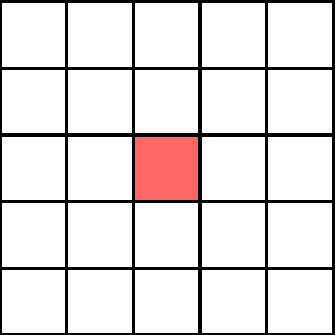
\includegraphics[width=0.9\textwidth]{replicator/00}
        \caption{Step 0}
    \end{subfigure}
    \begin{subfigure}{0.32\textwidth}
        \centering
        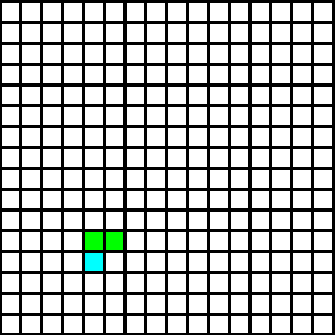
\includegraphics[width=0.9\textwidth]{replicator/01}
        \caption{Step 1}
    \end{subfigure}
    \begin{subfigure}{0.32\textwidth}
        \centering
        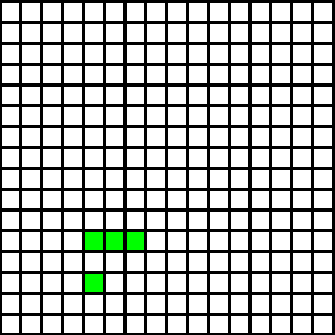
\includegraphics[width=0.9\textwidth]{replicator/02}
        \caption{Step 2}
    \end{subfigure}
    \par\bigskip
    \begin{subfigure}{0.32\textwidth}
        \centering
        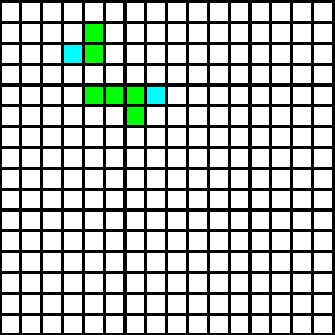
\includegraphics[width=0.9\textwidth]{replicator/03}
        \caption{Step 3}
    \end{subfigure}
    \begin{subfigure}{0.32\textwidth}
        \centering
        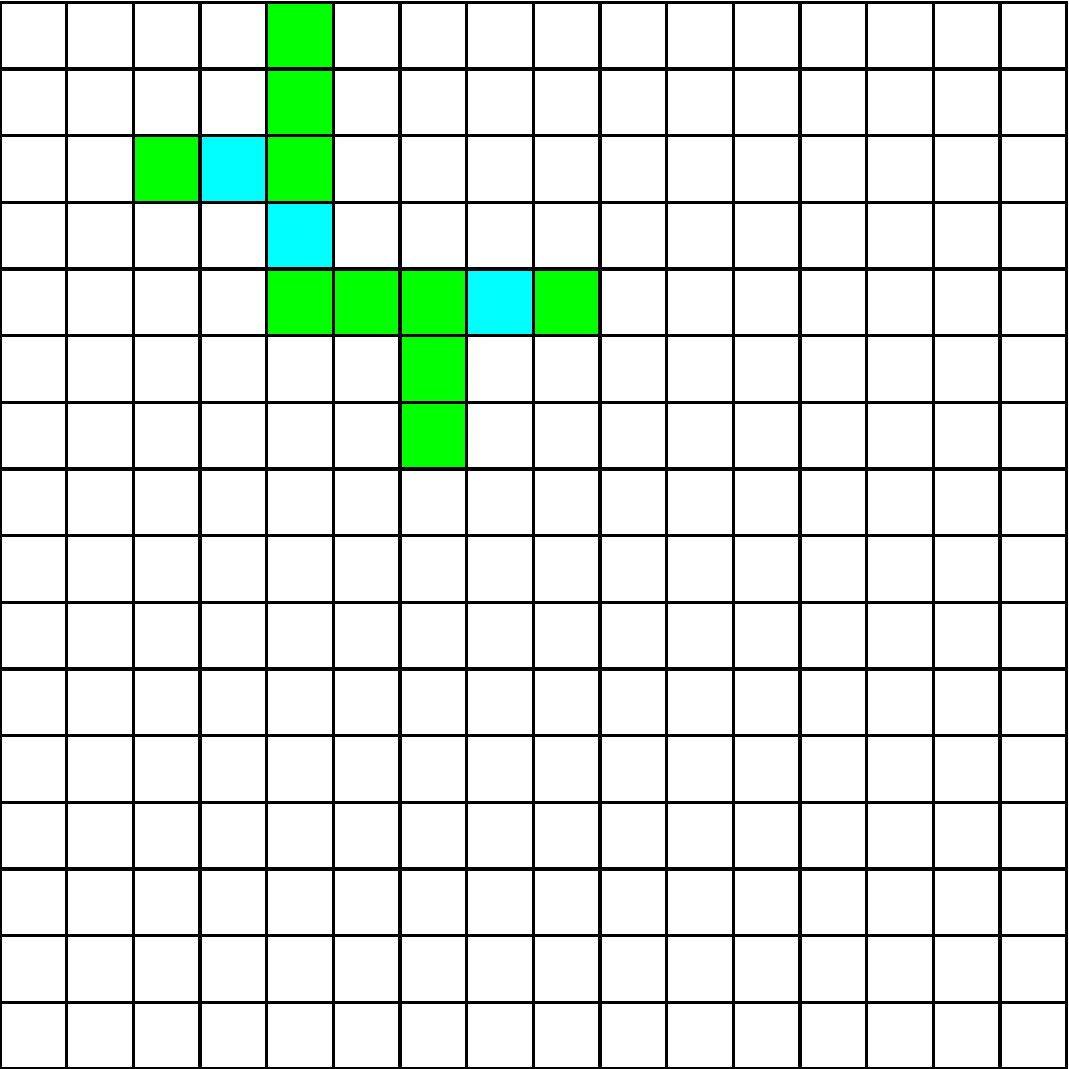
\includegraphics[width=0.9\textwidth]{replicator/04}
        \caption{Step 4}
    \end{subfigure}
    \begin{subfigure}{0.32\textwidth}
        \centering
        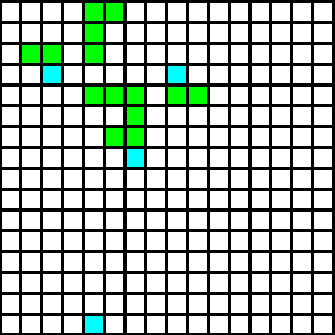
\includegraphics[width=0.9\textwidth]{replicator/05}
        \caption{Step 5}
    \end{subfigure}
    \par\bigskip
    \begin{subfigure}{0.32\textwidth}
        \centering
        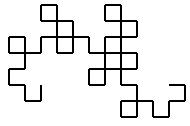
\includegraphics[width=0.9\textwidth]{replicator/06}
        \caption{Step 6}
    \end{subfigure}
    \begin{subfigure}{0.32\textwidth}
        \centering
        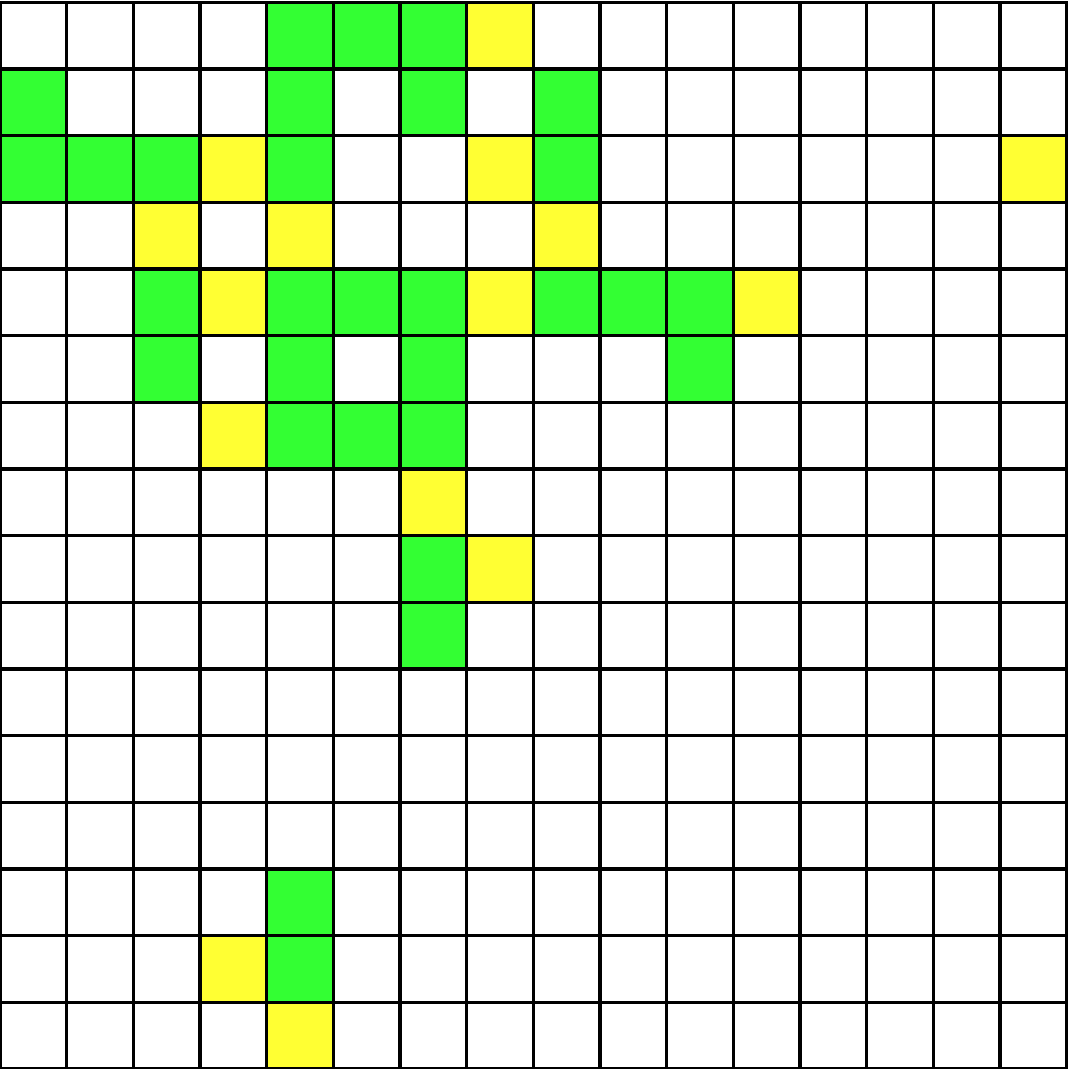
\includegraphics[width=0.9\textwidth]{replicator/07}
        \caption{Step 7}
    \end{subfigure}
    \begin{subfigure}{0.32\textwidth}
        \centering
        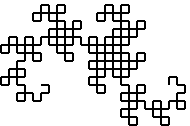
\includegraphics[width=0.9\textwidth]{replicator/08}
        \caption{Step 8}
    \end{subfigure}
    \par\bigskip
    \begin{subfigure}{0.32\textwidth}
        \centering
        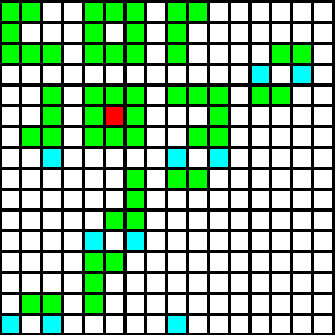
\includegraphics[width=0.9\textwidth]{replicator/09}
        \caption{Step 9}
    \end{subfigure}
    \begin{subfigure}{0.32\textwidth}
        \centering
        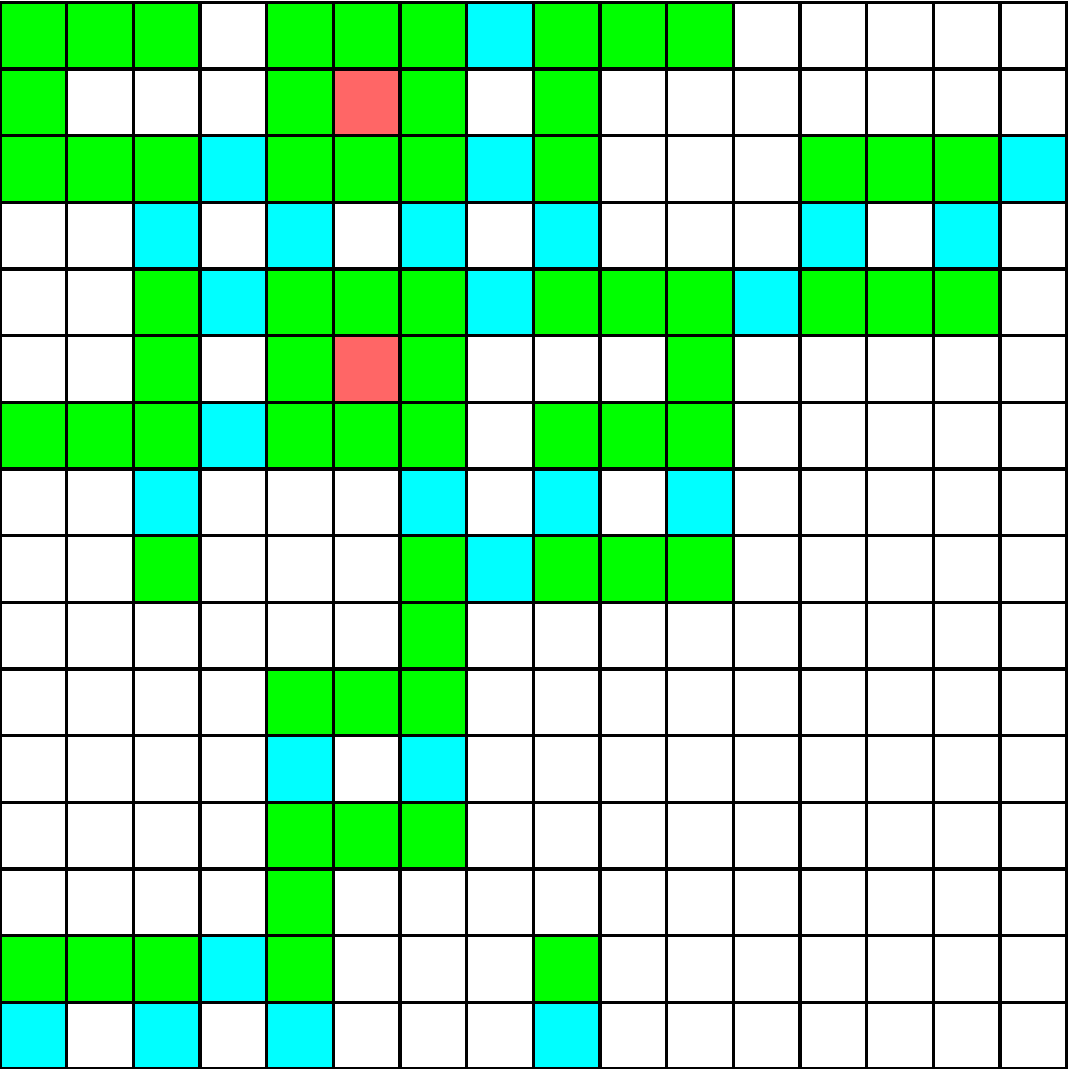
\includegraphics[width=0.9\textwidth]{replicator/10}
        \caption{Step 10}
    \end{subfigure}
    \begin{subfigure}{0.32\textwidth}
        \centering
        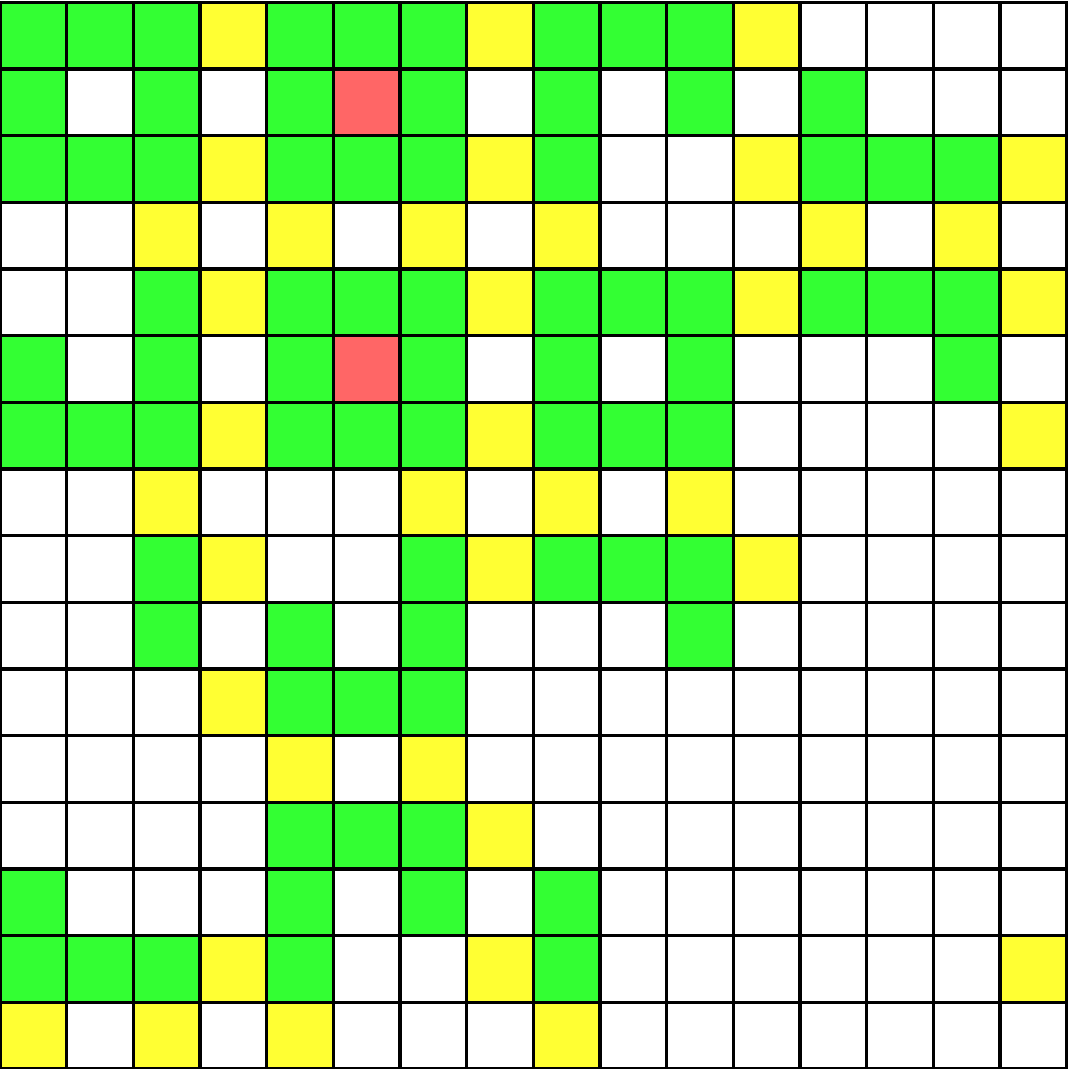
\includegraphics[width=0.9\textwidth]{replicator/11}
        \caption{Step 11}
    \end{subfigure}
\end{figure}

\begin{figure}[!ht]
    \ContinuedFloat
    \centering
    \begin{subfigure}{0.32\textwidth}
        \centering
        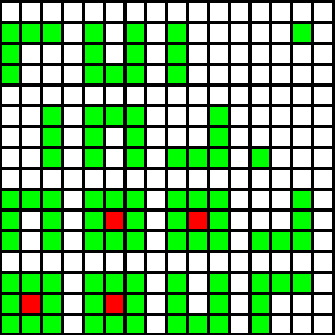
\includegraphics[width=0.9\textwidth]{replicator/12}
        \caption{Step 12}
    \end{subfigure}
    \begin{subfigure}{0.32\textwidth}
        \centering
        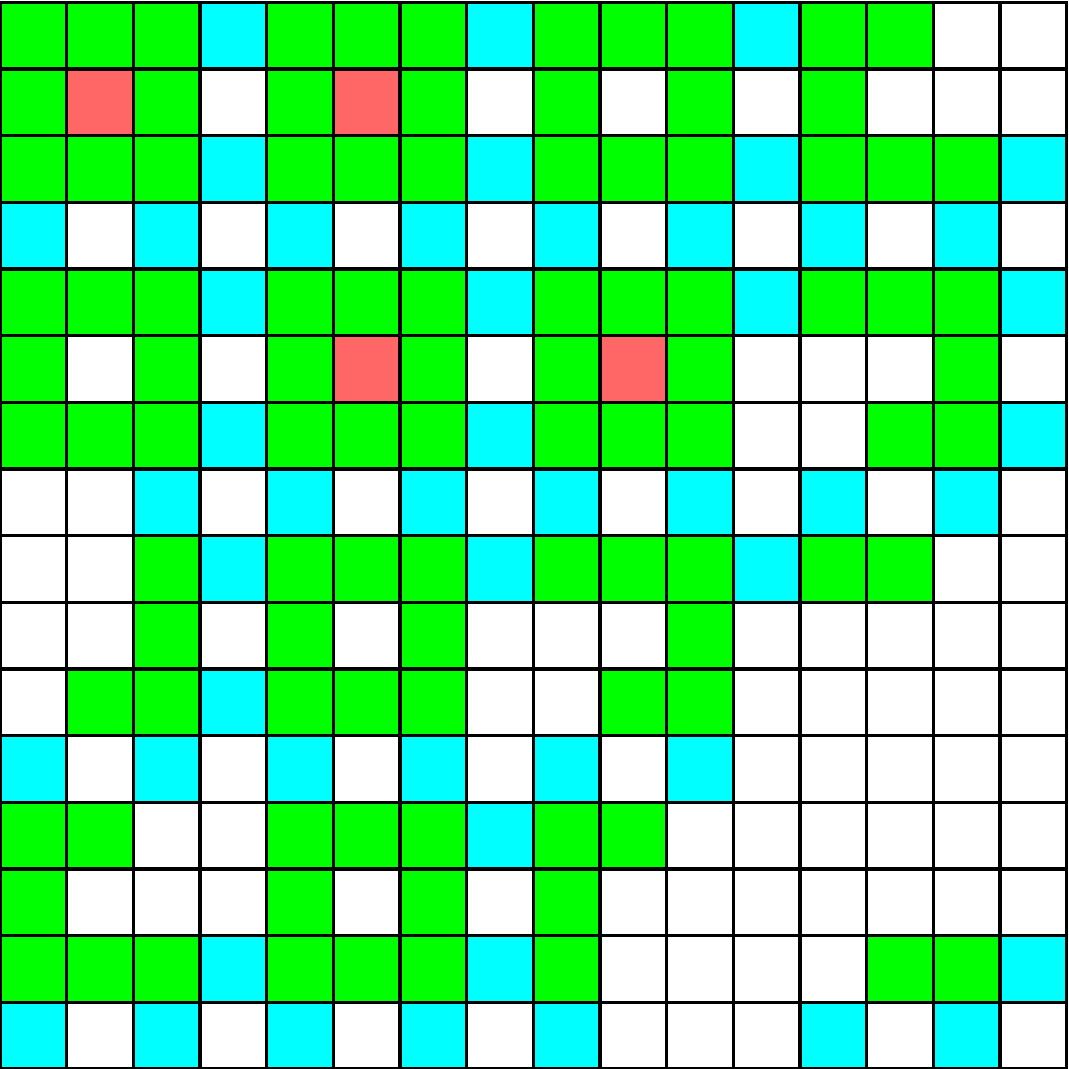
\includegraphics[width=0.9\textwidth]{replicator/13}
        \caption{Step 13}
    \end{subfigure}
    \begin{subfigure}{0.32\textwidth}
        \centering
        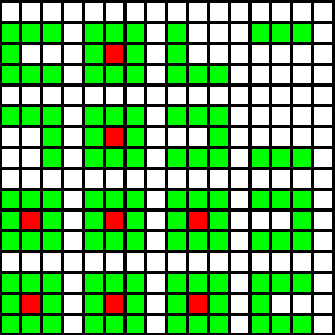
\includegraphics[width=0.9\textwidth]{replicator/14}
        \caption{Step 14}
    \end{subfigure}
    \par\bigskip
    \begin{subfigure}{0.32\textwidth}
        \centering
        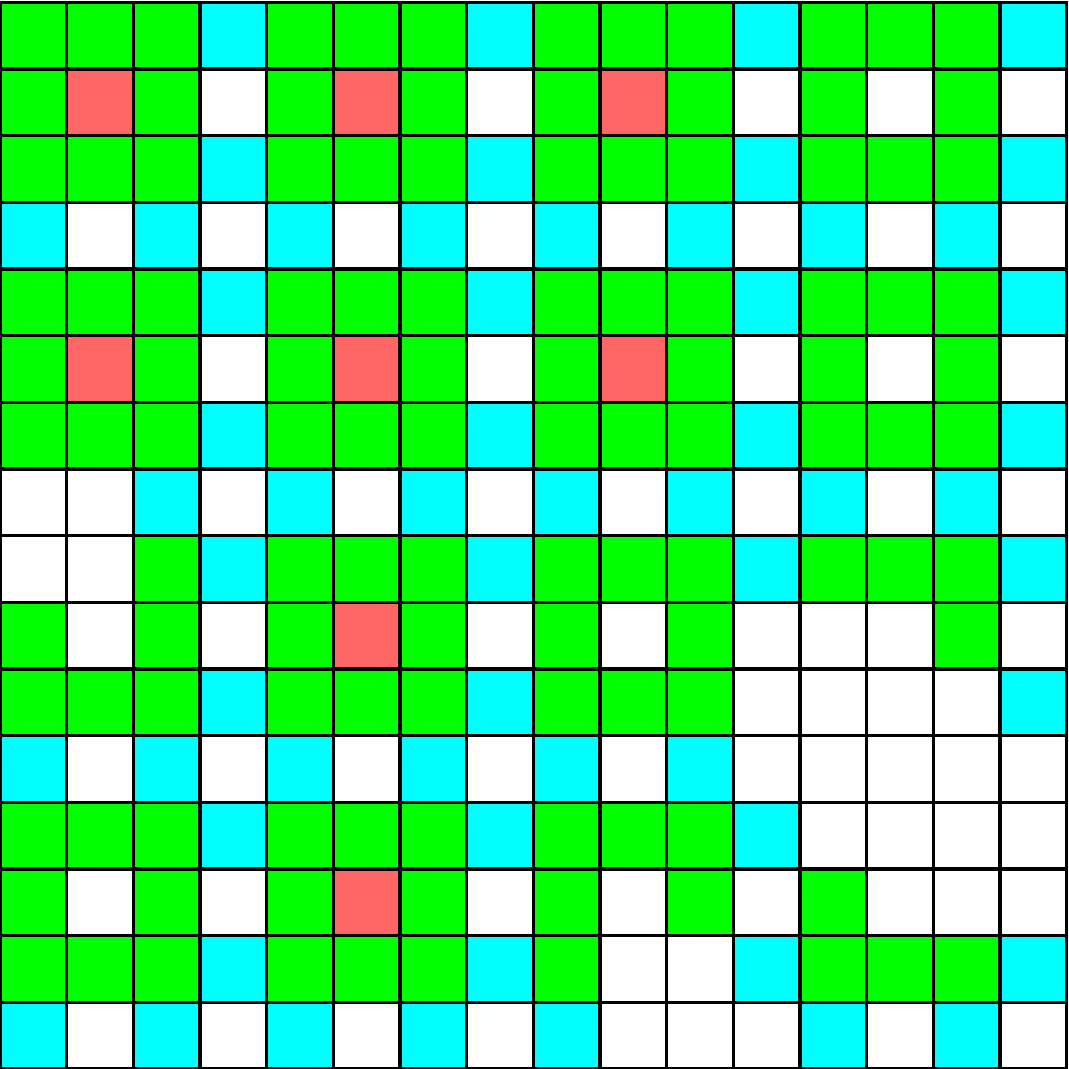
\includegraphics[width=0.9\textwidth]{replicator/15}
        \caption{Step 15}
    \end{subfigure}
    \begin{subfigure}{0.32\textwidth}
        \centering
        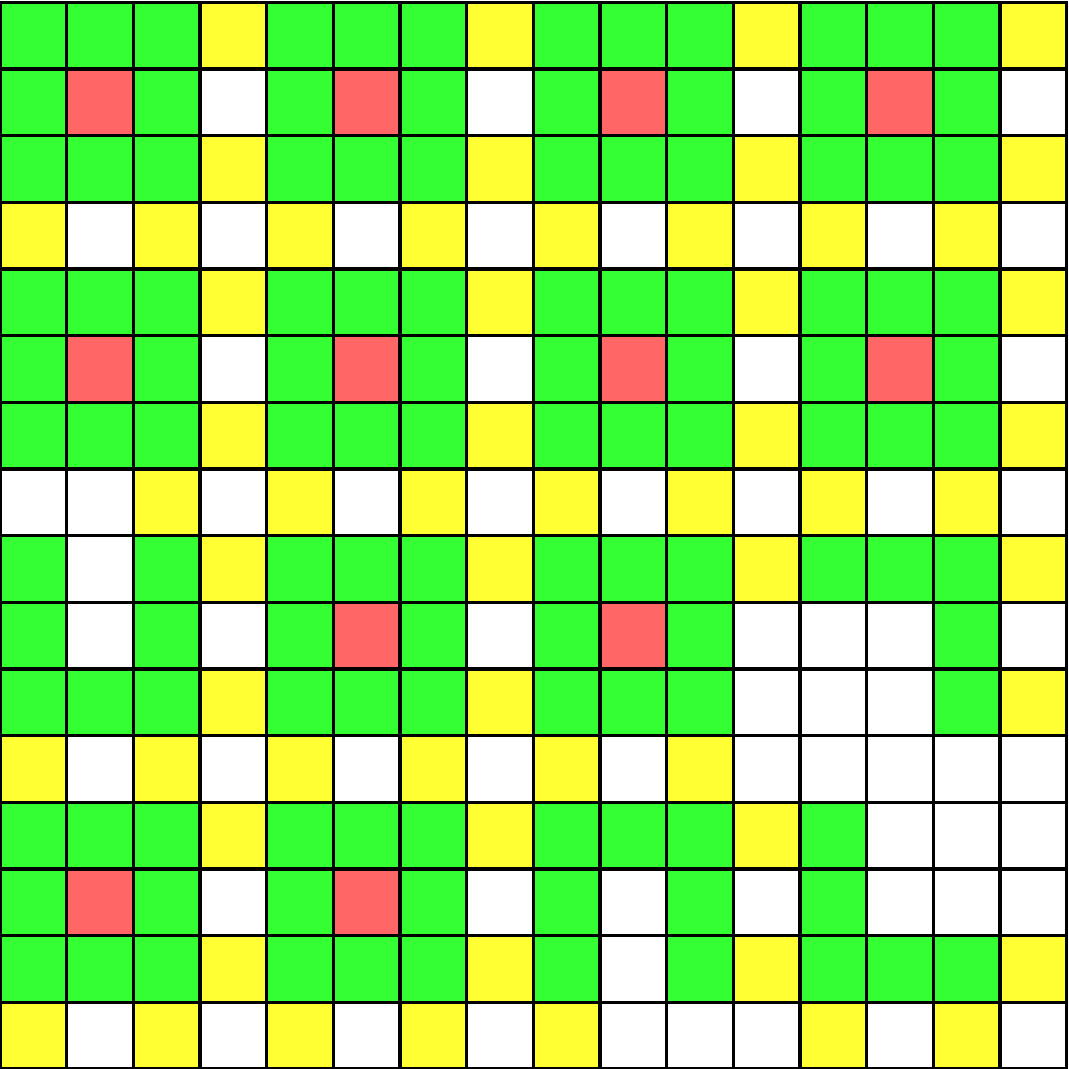
\includegraphics[width=0.9\textwidth]{replicator/16}
        \caption{Step 16}
    \end{subfigure}
    \begin{subfigure}{0.32\textwidth}
        \centering
        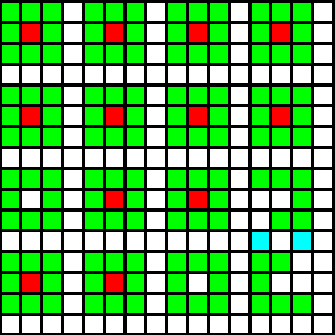
\includegraphics[width=0.9\textwidth]{replicator/17}
        \caption{Step 17}
    \end{subfigure}
    \par\bigskip
    \begin{subfigure}{0.32\textwidth}
        \centering
        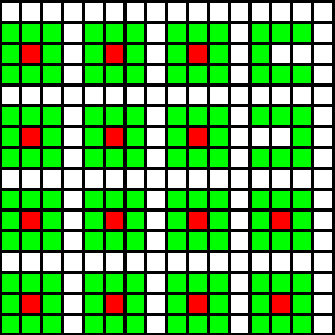
\includegraphics[width=0.9\textwidth]{replicator/18}
        \caption{Step 18}
    \end{subfigure}
    \begin{subfigure}{0.32\textwidth}
        \centering
        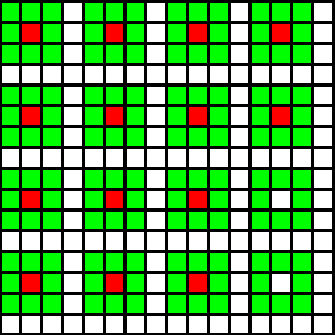
\includegraphics[width=0.9\textwidth]{replicator/19}
        \caption{Step 19}
    \end{subfigure}
    \begin{subfigure}{0.32\textwidth}
        \centering
        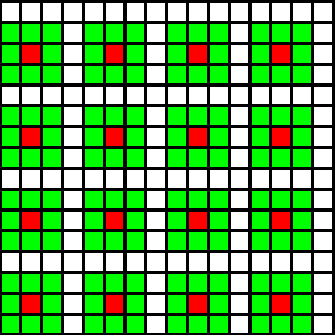
\includegraphics[width=0.9\textwidth]{replicator/20}
        \caption{Step 20}
    \end{subfigure}
    \caption[Replicator] {
        TODO
    }
    \label{fig:replicator}
\end{figure}

\TODO
Stacked demo
